% 目次の挿入
\tableofcontents
\newpage

% ヘッダーカスタマイズ
\pagestyle{fancy}
\fancyhf{}
\fancyhead[L]{DLITE3:Technology that supports people's lives without boundaries}
\renewcommand{\headrulewidth}{0pt}
\makeatletter
\let\ps@plain\ps@fancy
\makeatother
% ヘッダーの下に空白を追加
\setlength{\headsep}{20pt}

\chapter{はじめに}
\section{背景}
適当な例で本文を書いていくので、chapterやsectionを含め本文を自由に改変してください。\\
朝、目覚まし時計が鳴り目が覚めた後、目覚まし時計まで手が届かず止めるのが困難である。
\begin{figure}[h!]
  \centering
  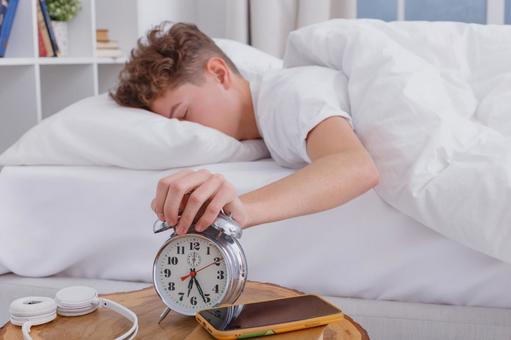
\includegraphics[width=0.8\textwidth]{pages/report/images/alarm-stopping.jpeg}
  \caption{目覚ましの停止が困難な図}
  \label{fig:sample}
\end{figure}
\writer{未来太郎}

\section{先行研究}
コダマ2024\cite{目覚まし時計を改造}によると、目覚まし時計を本体についているボタンとは別に停止する改造はすでに行われている。
しかし、その改造は目覚まし時計の本体に直接改造を加えるものであり、目覚まし時計の本体に直接改造を加えることは、目覚まし時計の保証が無効になる可能性がある。
また、ボタンの延長はケーブルで行われており、夜中布団から出るときなどに転倒の原因となる可能性があり、安全性に問題がある。
\writer{未来太郎}

\section{研究動機}
目覚まし時計がなることにより目が覚めた後、目覚まし時計を止めないことに快適な二度寝を楽しむことが出来ない。
そのため、目覚まし時計を止めることが容易になるような方法を考えることが必要であると考えた。
実際に、起床時にアラームで起きた際にどのような問題が生じるのかについてフィールドワークを行ったところ、布団から出て目覚まし時計を停止させることで目が覚めてしまい、快適な二度寝が出来ないことが判明した。
\writer{未来太郎}

\section{目的及び重要性}
本プロジェクトでは、視覚、聴覚の障害の有無に関わらず、自然を楽しむことのできる「自然エンタテインメントデバイス」を開発し、自然の新たな楽しみ方を実現する。
また、今年度以前も含め本プロジェクト学習では、多くの障害者支援デバイスの開発を行ってきている。
しかし、多くの開発されたデバイスは部分的には新規性があるものの、すでに近いデバイスやアプリ、サービスが存在しているものや、高価な機器を用いて開発されたさらに高機能なデバイスが存在しているものも少なくない。
そのため、本グループではブレインストーミングやフィールドワークから新たな価値を生み出すことのできるデバイスを目指した。
\writer{金子康一}

\chapter{関連研究}
\section{必要なスキル}
昨年度プロジェクト学習で使用されたスキル、技術は以下のようになっています。
\begin{itemize}
  \item M5Stack Core2
  \item unitv2 AIカメラ
  \item シリアル通信
  \item RetinaFace
  \item Object Recongnition
  \item V-Training
  \item UiFlow
  \item RaspberryPi 4
  \item OpenCV
  \item M5Stack 用 ToF 距離センサユニット
  \item M5Stack 用振動モータユニット
  \item M5Stack 用超音波測距ユニット
  \item 骨伝導イヤホン
\end{itemize}
\writer{金子康一}

\section{解決方法・手法}
目覚まし時計を止めるための方法として、ワイヤレスで目覚まし時計を操作する方法を考案する。
目覚まし時計が作動しし目が覚めた後、スマホを操作することで目覚まし時計の停止ボタンが遠隔で押されるようにする。
目覚まし時計本体の改造を行わなくても良いように、外付けが可能なデバイスを作成する。
\writer{未来太郎}

\chapter{本プロジェクト学習の目標}
\section{最終的な目標}
Rasberrypiを用いたカメラ型デバイスを開発し、画像と音の相互変換を行うことで、障害の有無に関わらず自然を楽しめるようにする。
具体的には、撮影した写真にあった曲を再生する機能と、録音した環境音にあったビジュアルアートを生成する。
それにより、自然の楽しみに新たな価値を生み出す。 
\writer{金子康一}

\chapter{目的を達成するための手法・手段}
\section{考案したアイデア}
\subsection{風景を音楽に変換する}
風景の写真をもとにAIが写真に合った曲を選曲し、Spotifyで曲を再生する。
このように風景を音楽に変換することで、視覚障害者でも音で風景を楽しむことを実現する。
\writer{金子康一}

\subsection{環境音をビジュアルアートに変換する}
録音した環境音をもとにAIがビジュアルアートを生成する。
このように環境音をビジュアルアートに変換することで、聴覚障害者でもビジュアルアートで環境音を楽しむことを実現する。
\writer{金子康一}

\section{新しい解決方法・手法}
\subsection{風景を音楽に変換する}
風景を音楽に変換するために、以下の二つの処理を行う。
\begin{enumerate}
  \item 画像に合った選曲を行う
  \item Spotifyに曲が存在するかを調べ再生する
\end{enumerate}
これらの機能を実現するために、図\ref{fig:image-to-select-music}、図\ref{fig:music-play}の技術構成で実装した。
\begin{figure}[h]
  \centering
  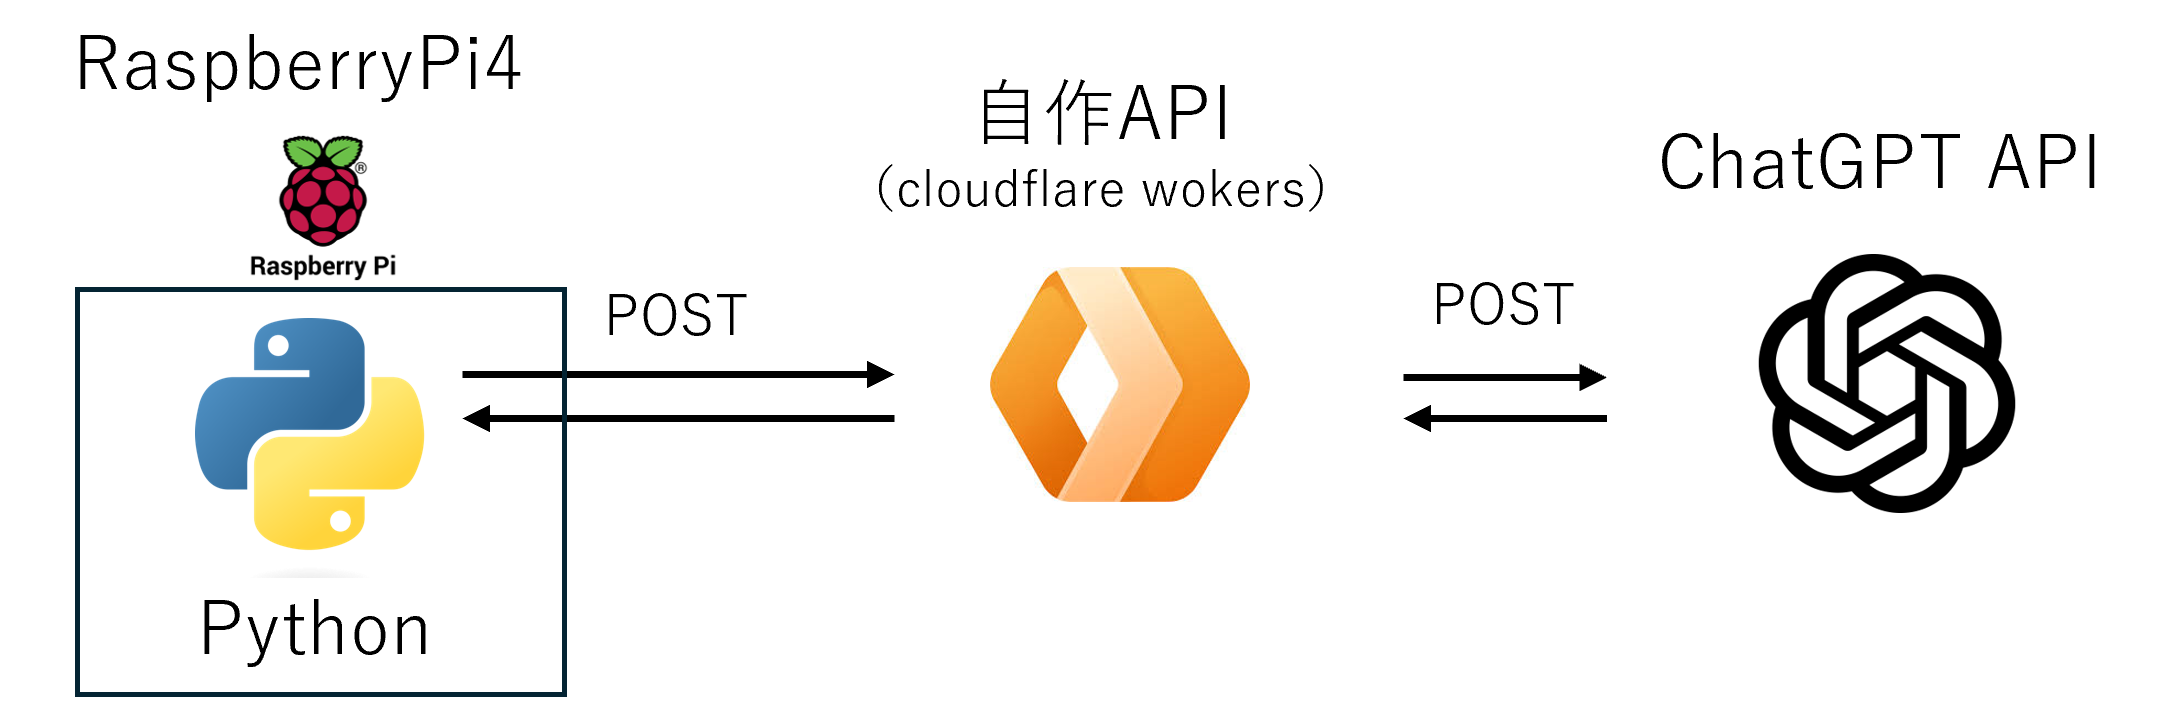
\includegraphics[width=0.8\textwidth]{pages/report/images/opeai-api.png}
  \caption{選曲機能の技術構成}
  \label{fig:image-to-select-music}
\end{figure}
\begin{figure}[h]
  \centering
  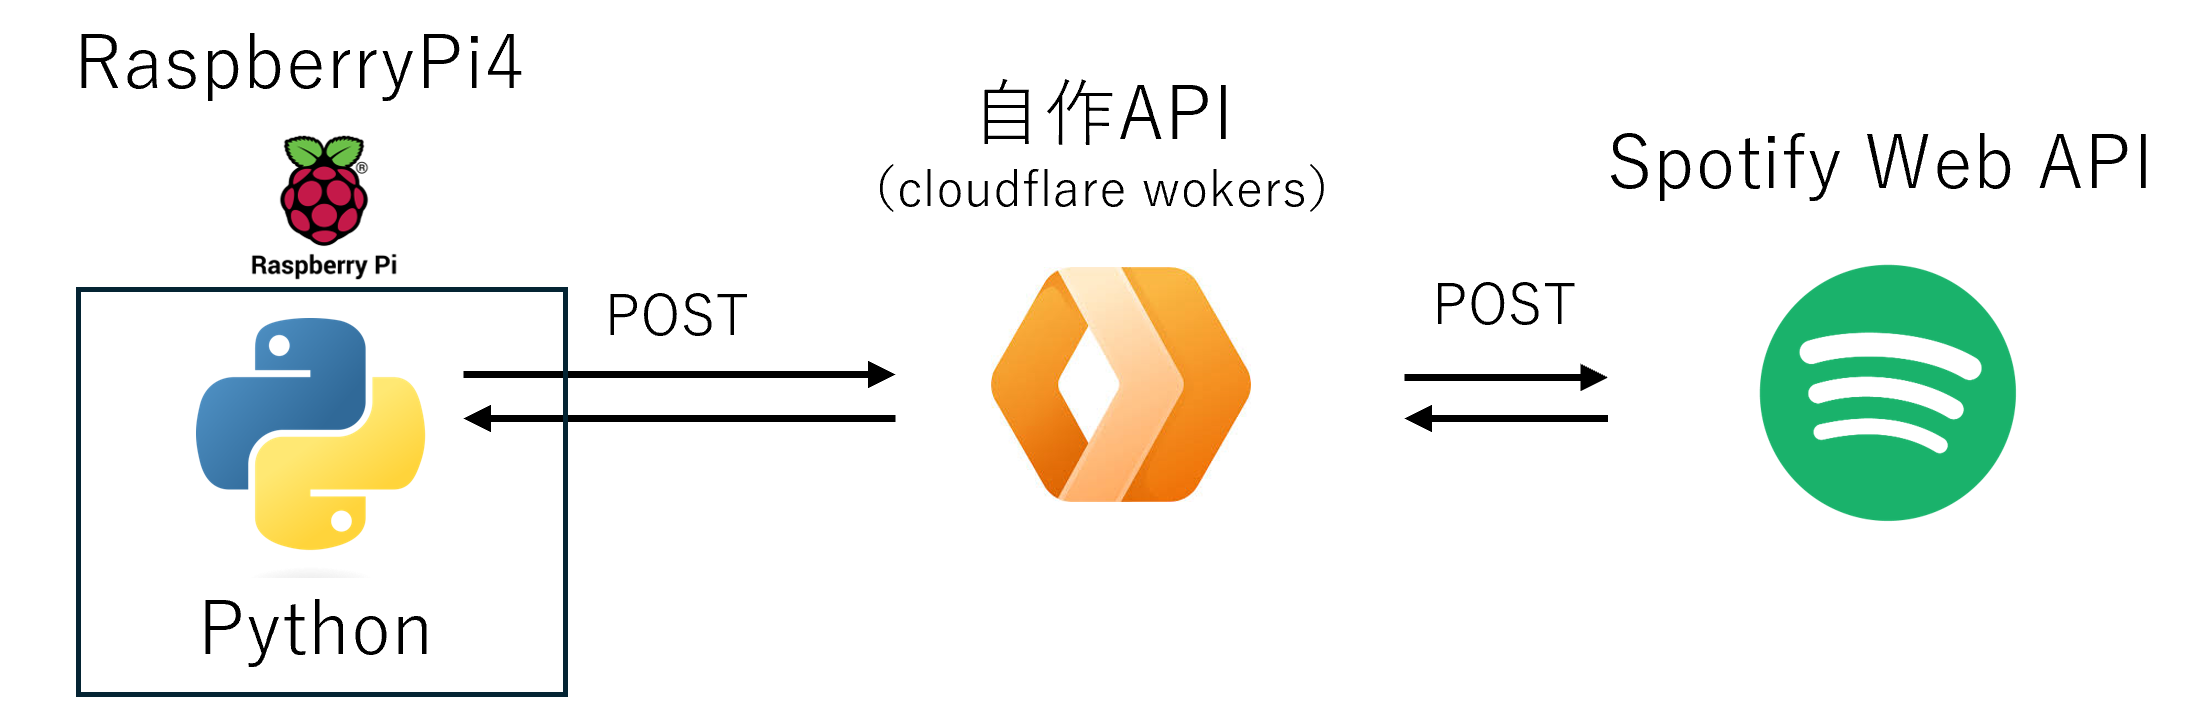
\includegraphics[width=0.8\textwidth]{pages/report/images/music-play.png}
  \caption{曲再生の技術構成}
  \label{fig:music-play}
\end{figure}
PythonとAPIの間にCloudflare WorkersでデプロイをしているHonoで作成した自作APIを挟んだ。
その理由として、PythonでAPIを使用する場合に実装に誤りがあり大量のリクエストを送信してしまうと、APIの利用制限やクレジットの大量消費がおきてしまう可能性がある。
そのため、自作のAPIを挟むことで、短時間にリクエストが来た場合にはAPIの利用を制限し、利用制限やクレジットの大量消費を防ぐことができた。
\writer{金子康一}

\subsection{環境音をビジュアルアートに変換する}
環境音をビジュアルアートに変換するために、以下の二つの処理を行う。
\begin{enumerate}
  \item Pythonで環境音の解析を行う
  \item 解析結果から画像生成のためのプロンプトを生成する
  \item 画像を生成する
\end{enumerate}
これらの機能を実現するために、図\ref{fig:generate-prompt}、図\ref{fig:generate-image}の技術構成で実装した。
\begin{figure}[h]
  \centering
  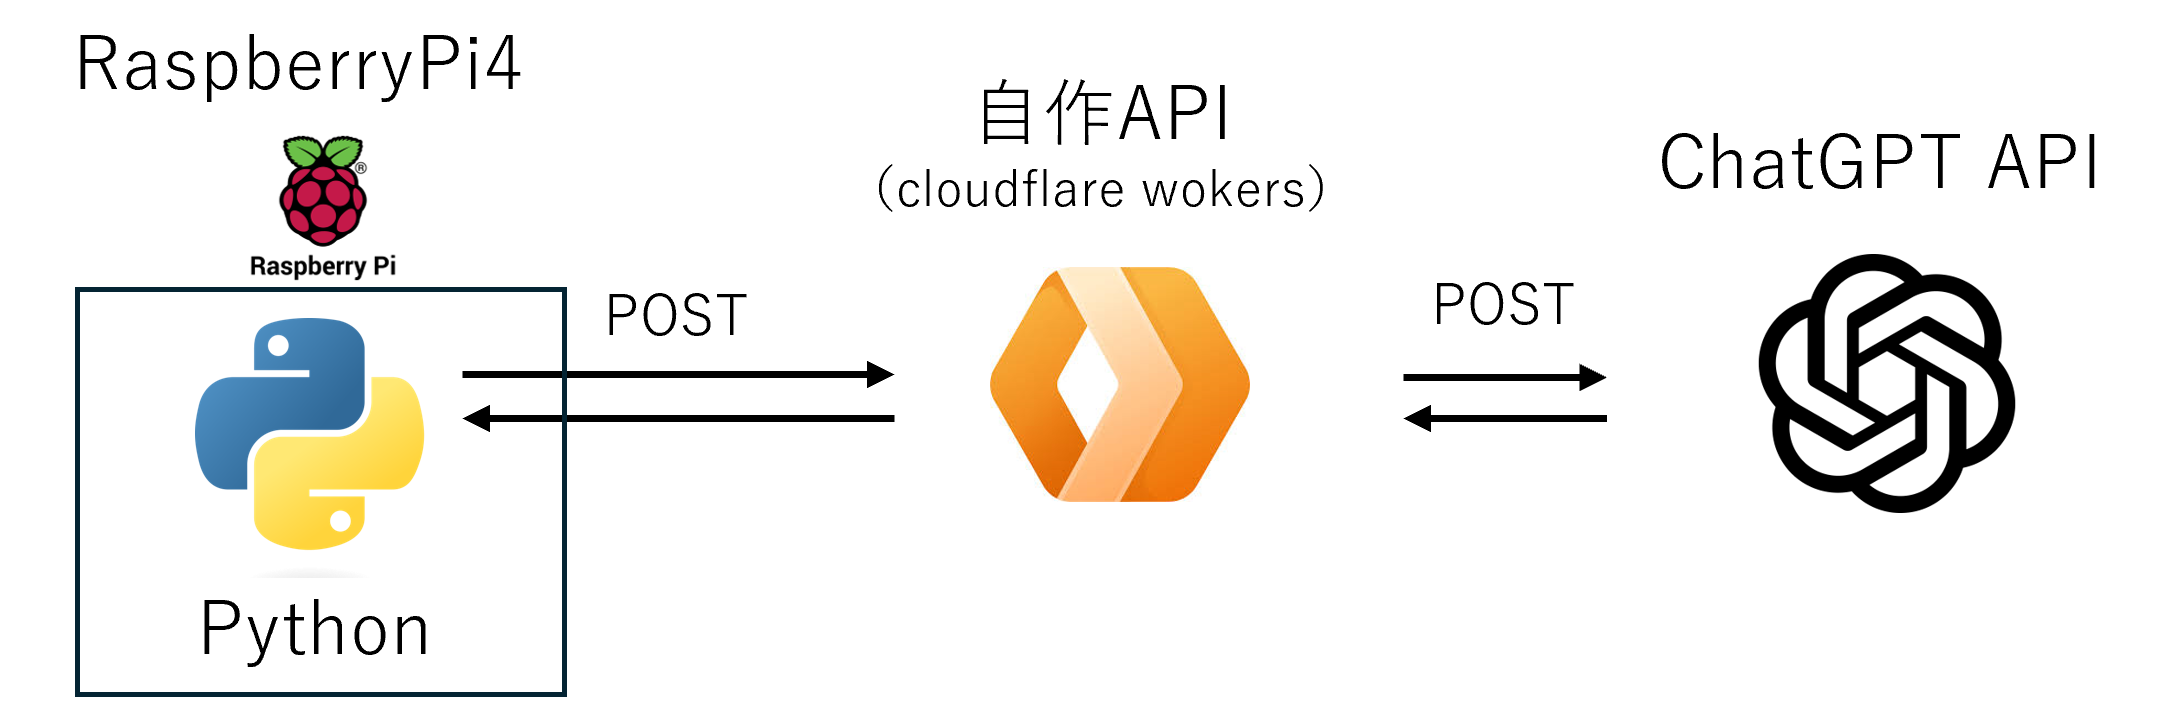
\includegraphics[width=0.8\textwidth]{pages/report/images/opeai-api.png}
  \caption{プロンプト生成の技術構成}
  \label{fig:generate-prompt}
\end{figure}
\begin{figure}[h]
  \centering
  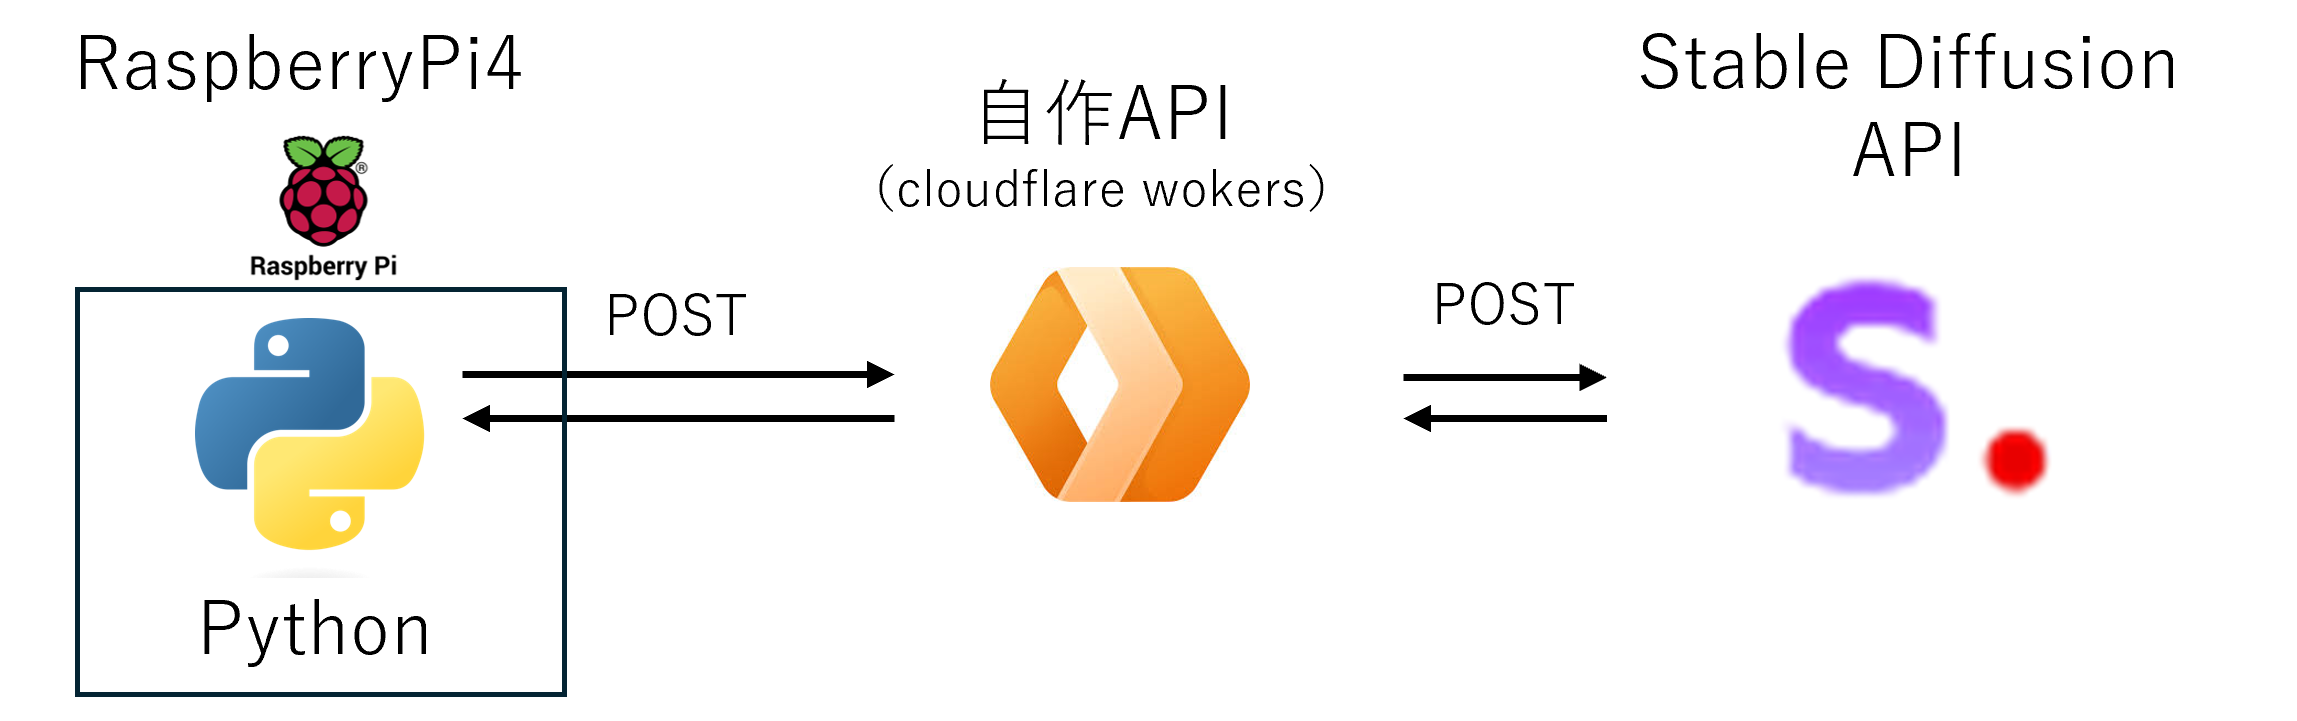
\includegraphics[width=0.8\textwidth]{pages/report/images/generate-image.png}
  \caption{画像生成の技術構成}
  \label{fig:generate-image}
\end{figure}
PythonとAPIの間にCloudflare WorkersでデプロイをしているHonoで作成した自作APIを挟んだ。
その理由として、PythonでAPIを使用する場合に実装に誤りがあり大量のリクエストを送信してしまうと、APIの利用制限やクレジットの大量消費がおきてしまう可能性がある。
そのため、自作のAPIを挟むことで、短時間にリクエストが来た場合にはAPIの利用を制限し、利用制限やクレジットの大量消費を防ぐことができた。
\writer{金子康一}

\section{用いる技術}
これらの機能を実現するために、以下の技術、スキルを用いた。
\begin{itemize}
  \item プログラム言語・フレームワーク
  \begin{itemize}
    \item Python
    \item Cpp
    \item TypeScript
    \item Hono
  \end{itemize}
  \item API
  \begin{itemize}
    \item OpenAI API
    \item Spotify Web API
    \item StableDiffusion API
  \end{itemize}
  \item HTTPメソッド
  \begin{itemize}
    \item HTTP GET
    \item HTTP POST
  \end{itemize}
  \item RaspberryPi 4
  \begin{itemize}
    \item GPIO
    \item I2C
    \item SPI
    \item カメラ
  \end{itemize}
  \item 電子回路制作
  \begin{itemize}
    \item 電子回路設計
    \item はんだ付け
    \item 圧着
  \end{itemize}
  \item 本体制作
  \begin{itemize}
    \item Fusion360
    \item CO2レーザーカッター
  \end{itemize}
\end{itemize}
\writer{金子康一}

\chapter{結果}
\section{主要な結果}
どんな結果が得られたのかを事実に基づいて述べる。
\writer{金子康一}

\chapter{考察}
\section{得られた成果}
本プロジェクト学習を通じてどのような成果を得られ、どのような効果が発生したのかについて考察する。
\writer{金子康一}

\section{妥当性}
得られた結果は妥当かどうかについて述べる。
\writer{金子康一}

\section{課題点}
用いた手法、技術では得られなかったことについて述べる。
\writer{金子康一}

\section{本学との関連性}
本学のカリキュラムや講義科目との関係や関連性について述べる。
\writer{金子康一}

\section{拡張性}
本プロジェクト学習を拡張することでどのような新たなテーマが考えられるかについて述べる。
\writer{金子康一}

\section{今後の展望}
今後の展望について述べる。
\writer{未来太郎}

\newpage\clearpage
\vspace*{-20pt}
\addcontentsline{toc}{chapter}{参考文献}  % 目次に「参考文献」を追加
\printbibliography[segment=\therefsegment,heading=subbibliography]
